\documentclass[a4paper,10pt,titlepage]{article}
\usepackage{graphicx} % Required for inserting images
\usepackage[margin=2cm]{geometry} % Adjust the margins
\usepackage{amsmath}
\usepackage{amssymb}
\numberwithin{equation}{subsection}
\usepackage{float}
\usepackage{bm}
\usepackage{wrapfig}

\title{
	\textbf{\huge{Modern Design of Control Systems}}\\
	\textit{Notes and Summary}}

\author{Gregorio Valenti}

\date{\textit{Polytechnic of Turin}, September 2024 - February 2025}

\begin{document}
	\maketitle

	\section{Feedback Control System Definition}
	\hspace{1cm}
	For this course, we will consider the model below to represent the system under study:
	
	\begin{figure}[H] % Use [H] to fix the position
		\centering
		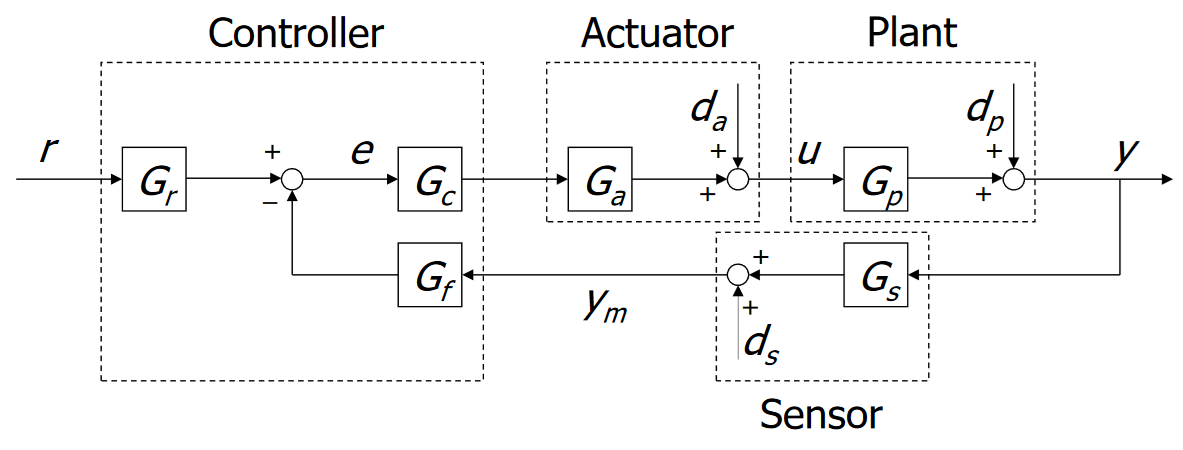
\includegraphics[scale=1]{images/feedback_loop_description.png}
		\caption{Feedback Control System}
		\label{fig:image1}
	\end{figure}

	With the following characteristics:
	\begin{enumerate}
		\item[$\bullet$] \textbf{Plant} $G_p$ with disturbance $d_p$
		\item[$\bullet$] \textbf{Actuator} $G_a$ with disturbance $d_a$
		\item[$\bullet$] \textbf{Sensor} $G_s$ with disturbance $d_s$
		\item[$\bullet$] \textbf{Feedback Controller} $G_c$ 	
	\end{enumerate}
	
	\section{Step response of prototype $\boldmath{2}^{\textbf{nd}}$ order system}
	For a prototype second order system with \textbf{Sensitivity} and \textbf{Complementary sensitivity} functions of the form:
	\begin{equation}
		T(s) = \dfrac{1}{1+\dfrac{2\zeta}{\omega_n}s+\dfrac{s^2}{\omega_n^2}} \quad ; \quad S(s) = \dfrac{s\left(\dfrac{2\zeta}{\omega_n}+\dfrac{s}{\omega_n^2}\right)}{1+\dfrac{2\zeta}{\omega_n}s+\dfrac{s^2}{\omega_n^2}}
	\end{equation}
	
	
	From the transient response indices for maximum overshoot $\hat{s}$, rise time $t_r$ and settling time $t_{s,\alpha\%}$, we can compute the system's damping coefficient, as well as constraints on the natural frequency and resonance peaks $T_p$ and $S_p$:
	\begin{enumerate}
		\item[$\bullet$] $\displaystyle \zeta = \frac{\left| \log (\hat{s}) \right|}{\sqrt{\pi^2 + \log^2 (\hat{s})}} \hfill (2.0.2)$
		\item[$\bullet$] $\displaystyle \omega_{n,tr} = \frac{1}{t_r\sqrt{1-\zeta^2}} \cdot (\pi - acos(\zeta)) \quad; \quad
		\omega_{n,t,s\alpha \%} = \frac{\log(\frac{100}{\alpha})}{t_{s,\alpha \%}\zeta} \hfill (2.0.3)$
		\item[$\bullet$] $\displaystyle \omega_c = \omega_n \sqrt{\sqrt{1+4\zeta^4}-2\zeta^2} \hfill (2.0.4)$
		\item[$\bullet$] $\displaystyle T_p = \frac{1}{2\zeta \sqrt{1-\zeta^2}} \quad; \quad S_p = \frac{2\zeta \sqrt{2+4\zeta^2+2\sqrt{1+8\zeta^2}}}{\sqrt{1+8\zeta^2}+4\zeta^2-1} \hfill (2.0.5)$
	\end{enumerate}
	
	\section{Steady-state Response to Polynomial Reference Inputs}
	Requirements on steady-state tracking error and steady-state errors in the presence of polynomial disturbances can be translated into constraints on the Sensitivity function.
	Therefore, by first writing $S(s) = s^{\nu+p}S^*(s)$, we can apply the final value theorem to each expression as described in the following subsections.
	\subsection{Tracking Error}
	\subsubsection{Problem formulation}
	The \textbf{tracking error} is defined as:
	\begin{equation}
		e_r(t) = y_d(t)-y_r(t) = K_dr(t)-y_r(t)
	\end{equation}
	Applying the \textbf{final value theorem} leads to:
	\begin{align}
		\left| e_r^\infty \right| &= \displaystyle\lim_{t\to\infty} 	\left|e_r(t)\right| = \displaystyle\lim_{s\to0}s \left|e_r(s)\right| = \displaystyle\lim_{s\to0}s \left|K_dr(s)-y_r(s)\right| = \nonumber \\
		&= \displaystyle\lim_{s\to0}s \left|G_{re}(s)r(s)\right| = 	\displaystyle\lim_{s\to0}s \left|S(s)K_dr(s)\right| = \nonumber \\
		&= \displaystyle\lim_{s\to0}s 	\left|s^{\nu+p}S^*(s)K_d\dfrac{h!R_0}{s^{h+1}}\right| =
		\begin{cases}
			0, & \text{if } \nu+p>h \\
			\left|S^*(0)K_dh!R_0\right|, & \text{if } \nu+p = h
		\end{cases}
	\end{align}
	The given system type is then $\nu+p$.
	\subsubsection{Conclusions}
	Considering the specification $\left|e_r^\infty\right| \leq \rho_r  $, we obtain the following result:
	\begin{enumerate}
		\item[$\bullet$] case $\rho_r=0 \implies S(s)$ must have a zero at $s=0$ with multiplicity greater than $h \implies$ We have no constraint on $\left|S^*(0)\right| $ 
		\item[$\bullet$] case $\rho_r>0 \implies S(s)$ must have a zero at $s=0$ with multiplicity $h \implies$ We have the following constraint:
		\begin{equation}
			\left|S^*(0)\right| \leq \dfrac{\rho_r}{K_dh!R_0}	
		\end{equation}
	\end{enumerate}
	
	\subsection{Error due to Generic Polynomial Disturbances $\bm{d(t)}$}
	\subsubsection{Problem formulation}
	The \textbf{output error} due to the generic disturbance $d(t)$ is the contribution of the disturbance to the output $y(t)$:
	\begin{equation}
		e_d(t) = y_d(t)
	\end{equation}
	
	\subsubsection{Polynomial disturbance $\bm{d_a(t)}$}
	Applying the \textbf{final value theorem} leads to:
	\begin{align}
		\left| e_{d_a}^\infty \right| &= \displaystyle\lim_{t\to\infty} 	\left|e_{d_a}(t)\right| = \displaystyle\lim_{s\to0}s \left|e_{d_a}(s)\right| = \displaystyle\lim_{s\to0}s \left|y_{d_a}(s)\right| = \displaystyle\lim_{s\to0}s \left| S(s)G_p(s)d_a(s) \right| = \nonumber \\
		&= \displaystyle\lim_{s\to0} 	\left|s^{\nu+p+1}S^*(s)G_p(s)\dfrac{h!D_{a0}}{s^{h+1}}\right| = \displaystyle\lim_{s\to0} \left|s^{\nu+1}S^*(s)K_p\dfrac{h!D_{a0}}{s^{h+1}}\right| =
		\begin{cases}
			0, & \text{if } \nu>h \\
			\left|S^*(0)K_ph!D_{a0}\right|, & \text{if } \nu = h
		\end{cases}
	\end{align}
	We then obtain two cases as before:
	\begin{enumerate}
		\item[$\bullet$] case $\rho_a=0 \implies S(s)$ must have a zero at $s=0$ with multiplicity greater than $h \implies$ We have no constraint on $\left|S^*(0)\right| $ 
		\item[$\bullet$] case $\rho_a>0 \implies S(s)$ must have a zero at $s=0$ with multiplicity $h \implies$ We have the following constraint:
		\begin{equation}
			\left|S^*(0)\right| \leq \dfrac{\rho_a}{K_ph!D_{a0}}	
		\end{equation}
	\end{enumerate}
	
	\subsubsection{Polynomial disturbance $\bm{d_p(t)}$}
	Applying the \textbf{final value theorem} leads to:
	\begin{align}
		\left| e_{d_p}^\infty \right| &= \displaystyle\lim_{t\to\infty} 	\left|e_{d_p}(t)\right| = \displaystyle\lim_{s\to0}s \left|e_{d_p}(s)\right| = \displaystyle\lim_{s\to0}s \left|y_{d_p}(s)\right| = \displaystyle\lim_{s\to0}s \left| S(s)d_p(s) \right| = \nonumber \\
		&= \displaystyle\lim_{s\to0}	\left|s^{\nu+p+1}S^*(s)\dfrac{h!D_{p0}}{s^{h+1}}\right| =
		\begin{cases}
			0, & \text{if } \nu+p>h \\
			\left|S^*(0)h!D_{p0}\right|, & \text{if } \nu+p = h
		\end{cases}
	\end{align}
	We then obtain two cases as before:
	\begin{enumerate}
		\item[$\bullet$] case $\rho_p=0 \implies S(s)$ must have a zero at $s=0$ with multiplicity greater than $h \implies$ We have no constraint on $\left|S^*(0)\right| $ 
		\item[$\bullet$] case $\rho_p>0 \implies S(s)$ must have a zero at $s=0$ with multiplicity $h \implies$ We have the following constraint:
		\begin{equation}
			\left|S^*(0)\right| \leq \dfrac{\rho_p}{h!D_{p0}}	
		\end{equation}
	\end{enumerate}
	
	\section{Steady-state Response to Sinusoidal Disturbances}
	\subsection{Output disturbance $\bm{d_p(t)}$}
	The focus is on the class of sinusoidal signals of the following type:
	\begin{equation}
		d_p = a_p\sin(\omega_pt) \quad \forall\omega_p\leq\omega_p^+ \quad \text{given } a_p \text{ and } w_p^+
	\end{equation}
	The output at steady-state is required to be bounded by a given constant:
	\begin{equation}
		\left| e_{d_p}^\infty \right| = \left| y_{d_p}^\infty \right| \leq \rho_p \quad \text{with } \rho_p>0
	\end{equation}
	The specification leads to a \textbf{frequency domain constraint} on the Sensitivity function $S(s)$ which can be computed as follows:
	\begin{align}
		\left| e_{d_p}^\infty \right| &= \left| y_{d_p}^\infty \right| = \left| a_pS(j\omega_p)\sin(\omega_pt+\varphi_p) \right| \leq a_p\left|S(j\omega_p)\right| \leq \rho_p \nonumber \\
		&\implies \left|S(j\omega_p)\right| \leq \dfrac{\rho_p}{a_p} = M_S^{LF} \quad \forall\omega_p \leq \omega_p^+
	\end{align}
	
	\subsection{Sensor Noise $\bm{d_s(t)}$}
	The focus is on the class of sinusoidal signals of the following type:
	\begin{equation}
		d_s = a_s\sin(\omega_st) \quad \forall\omega_s\geq\omega_s^- \quad \text{given } a_s \text{ and } w_s^-
	\end{equation}
	The output at steady-state is required to be bounded by a given constant:
	\begin{equation}
		\left| e_{d_s}^\infty \right| = \left| y_{d_s}^\infty \right| \leq \rho_s \quad \text{with } \rho_s>0
	\end{equation}
	The specification leads to a \textbf{frequency domain constraint} on the Complementary Sensitivity function $T(s)$ which can be computed as follows:
	\begin{align}
		\left| e_{d_s}^\infty \right| &= \left| y_{d_s}^\infty \right| = \left| a_sT(j\omega_s)\dfrac{1}{G_s}\sin(\omega_st+\varphi_s) \right| \leq a_s\left|T(j\omega_s)\dfrac{1}{G_s}\right| \leq \rho_s \nonumber \\
		&\implies \left|T(j\omega_s)\right| \leq \dfrac{\rho_sG_s}{a_s} = M_T^{HF} \quad \forall\omega_s \leq \omega_s^-
	\end{align}
	
	
	\section{Weighting Functions Construction}
	\subsection{Rational Approximation of Frequency Constraints}
	\begin{enumerate}
		\item[$\bullet$] Rational functions of the Laplace variable s are used to approximate the frequency domain constraints on $S(s)$ and $T(s)$.
		\item[$\bullet$] The parameters of the approximating functions (steady-state gain zeros and poles) can be moved to get the desired result.
		\item[$\bullet$] \textbf{Butterworth polynomials} can be used either as denominator or numerator of the approximating rational function to effectively retain constraints on different frequency ranges.
	\end{enumerate}
	\begin{table}[H] % Use [H] to fix position
		\begin{minipage}{0.52\textwidth} % Adjust width as needed
			\centering
			\begin{tabular}{|c|c|}
				\hline
				\textbf{Polynomial Order} & \textbf{Polynomial Structure} \\ \hline
				0 & $1$ \\ \hline
				1 & $1+\dfrac{s}{\omega_a}$ \\ \hline
				2 & $1+\dfrac{2\zeta}{\omega_a}s+\left(\dfrac{s}{\omega_a}\right)^2$ \\ \hline
				3 & $1+\dfrac{2}{\omega_a}s+2\left(\dfrac{s}{\omega_a}\right)^2+\left(\dfrac{s}{\omega_a}\right)^3$ \\ \hline
			\end{tabular}
			\caption{Butterworth Polynomials}
			\label{tab:polynomial_table}
		\end{minipage}
		\hfill
		\begin{minipage}{0.5\textwidth}
			\raggedright
			\vspace{-54pt}
			The \textbf{key property} of Butterworth polynomials is that, when used in the numerator or denominator of a rational function, they increase or decrease the frequency response magnitude by 3 dB respectively, at the frequency $\omega_a$, regardless of the polynomial's order.
		\end{minipage}
	\end{table}
	The goal is to obtain the \textbf{rational functions} $\bm{W_S^{-1}(s)}$ \textbf{and} $\bm{W_T^{-1}(s)}$ such that the constraints derived above are satisfied.
	\begin{enumerate}
		\item[$\bullet$] Considering low frequencies we have:
		\begin{equation}
			\left| W_S^{-1}(j\omega) \right| \leq M_S^{LF} \quad \forall 	\omega_p\leq\omega_p^+ \quad ; \quad \max_\omega \left| W_S^{-1}(\infty) \right| \leq S_{p0}
		\end{equation}	
		\item[$\bullet$] Considering high frequencies we have:
		\begin{equation}
			\left| W_T^{-1}(j\omega) \right| \leq M_T^{HF} \quad \forall 	\omega_s\geq\omega_s^- \quad ; \quad \max_\omega \left| W_T^{-1}(j\omega) \right| \leq T_{p0} \implies \left| W_T^{-1}(0) \right| = T_{p0}
		\end{equation}
	\end{enumerate}
	
	\begin{figure}[htbp]
		\centering
		% First minipage for the first image
		\begin{minipage}{0.45\textwidth} % Adjust the width as needed
			\centering
			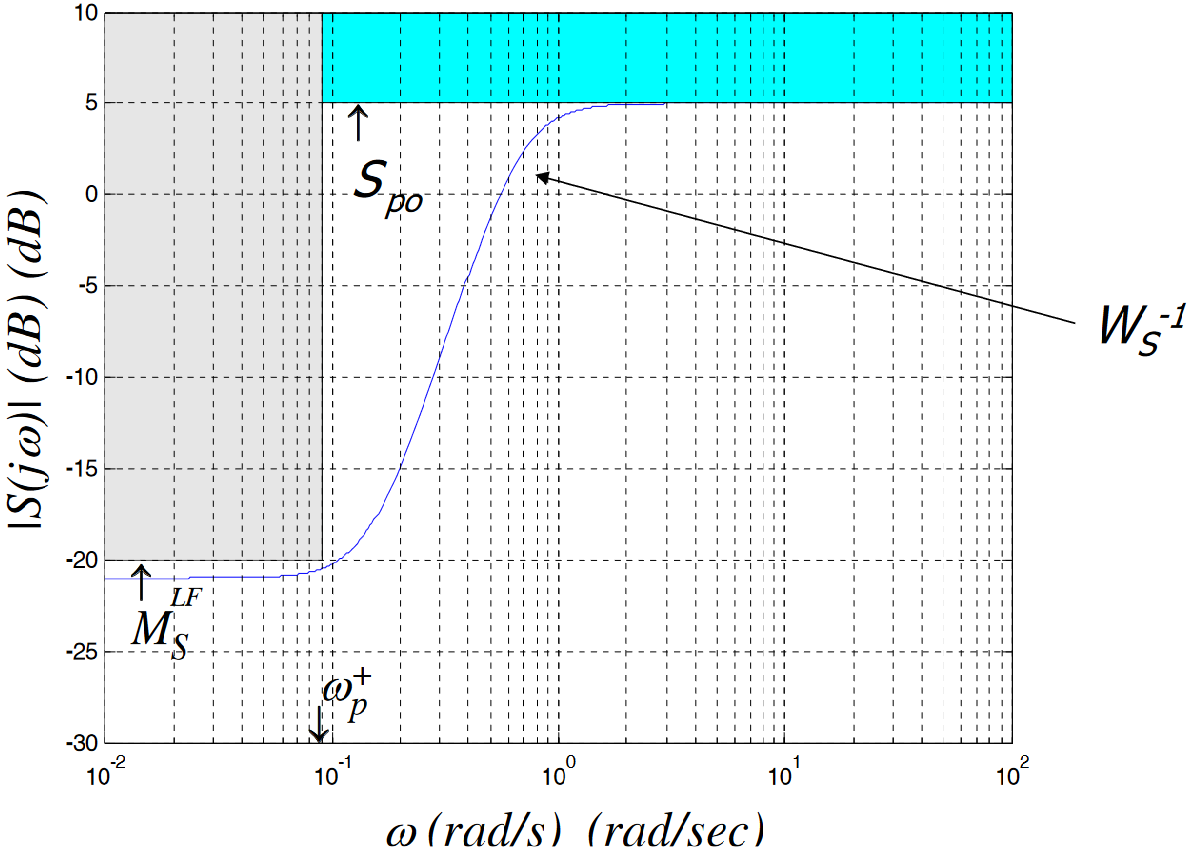
\includegraphics[width=\linewidth]{images/Approximation_W_S.png}
			\caption{Weighting Function $W_S^{-1}$}
			\label{fig:image2}
		\end{minipage}
		\hfill % Adds horizontal space between the images
		% Vertical line
		\vrule width 0.5pt % Adjust the width of the line as needed
		\hfill % Adds horizontal space before the second image
		% Second minipage for the second image
		\begin{minipage}{0.45\textwidth} % Adjust the width as needed
			\centering
			\vspace{0pt}
			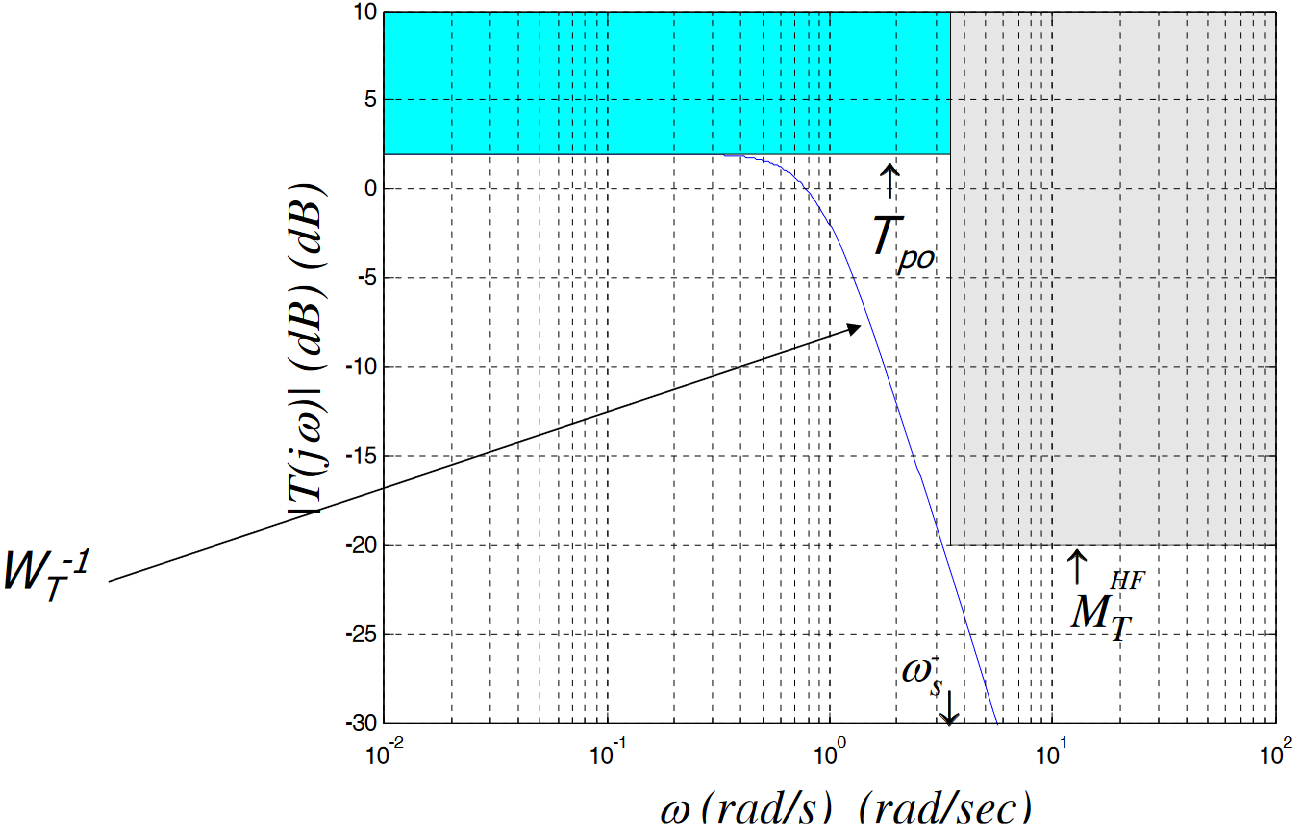
\includegraphics[width=1.135\linewidth]{images/Approximation_W_T.png}
			\caption{Weighting Function $W_T^{-1}$}
			\label{fig:image3}
		\end{minipage}
	\end{figure}
	
	\section{Performance Specification as $\bm{H_\infty}$ Norm Constraints}
	\subsection{$\bm{H_\infty}$ Norm Definition}
	By defining:
	\begin{enumerate}
		\item[$\bullet$] $W_S(s)$ as the inverse of the rational approximation of the frequency domain constraints on the Sensitivity function S(s)
		\item[$\bullet$] $W_T(s)$ as the inverse of the rational approximation of the frequency domain constraints on the Complementary Sensitivity function T(s)
	\end{enumerate}
	Design constraints obtained from the considered performance requirements can be written in the following compact form:
	\begin{equation}
		\left| W_S(j\omega)S(j\omega) \right| \leq 1 \quad ; \quad \left| W_T(j\omega)T(j\omega) \right| \leq 1 \quad \forall\omega	
	\end{equation}
	The $\bm{H_\infty}$ \textbf{norm} of a SISO LTI system with transfer function $H(s)$ is defined as:
	\begin{equation}
		\left\lVert H(s) \right\rVert_\infty \triangleq \max_\omega \left| H(j\omega) \right|
	\end{equation}
	It is now possible to rewrite the design constraints obtained above in terms of the weighted $H_\infty$ norm of $S(s)$ and $T(s)$:
	\begin{equation}
		\left\lVert W_S(s)S(s) \right\rVert_\infty \leq 1 \quad ; \quad \left\lVert W_T(s)T(s) \right\rVert_\infty \leq 1
	\end{equation}

	\section{Unstructured Uncertainty Modelling}
	Mathematical models cannot exactly describe a physical process, irrespective of their complexity. Thus, model uncertainty has to be taken into account when a mathematical model is used to analyse the behaviour of a system, or to design a feedback control system.
	\textbf{Unstructured uncertainty} comes into play when complete ignorance regarding the order and the phase behaviour of the system is assumed, and parametric uncertainty can also be described by means of unstructured model sets.
	\subsection{Uncertainty Model Sets}
	The following four uncertainty model sets will be considered, in which:
	\begin{enumerate}
		\item[$\bullet$] $G_p(s) $ is the transfer function of the generic member of the uncertainty set. 
		\item[$\bullet$] $G_{pn}(s)$ is the transfer function of the \textbf{nominal model}.
		\item[$\bullet$] $\Delta(s)$ represents any possible transfer function whose $H_\infty$ norm is less than 1.
		\item[$\bullet$] $W_u(s)$ is a \textbf{weighting function} which accounts for the size of the uncertainty.
	\end{enumerate} 
	Particular focus will be on the second set.
	\subsubsection{Additive Uncertainty}
	The additive uncertainty model set is defined as:
	
	\begin{equation}
		M_a = \left\{ G_p(s): G_p(s)=G_{pn}(s)+W_u(s)\Delta(s), \left\lVert\Delta(s)\right\rVert_\infty \leq1 \right\}
	\end{equation}
	where, by construction, the following condition must be satisfied by the weighting function $W_u(s)$:
	\begin{equation}
		\left\lVert \dfrac{G_p(s)-G_{pn}(s)}{W_u(s)} \right\rVert_\infty = \left\lVert \Delta(s) \right\rVert_\infty \leq 1
	\end{equation}
	which is equivalent to:
	\begin{equation}
		\left| G_p(j\omega)-G_{pn}(j\omega) \right| \leq \left| W_u(j\omega) \right| \quad \forall \omega
	\end{equation}
	
	Below is an example of the frequency response of $W_u(j\omega)$ for an additive uncertainty model set:
	
	\begin{figure}[H] % Use [H] to fix the position
		\centering
		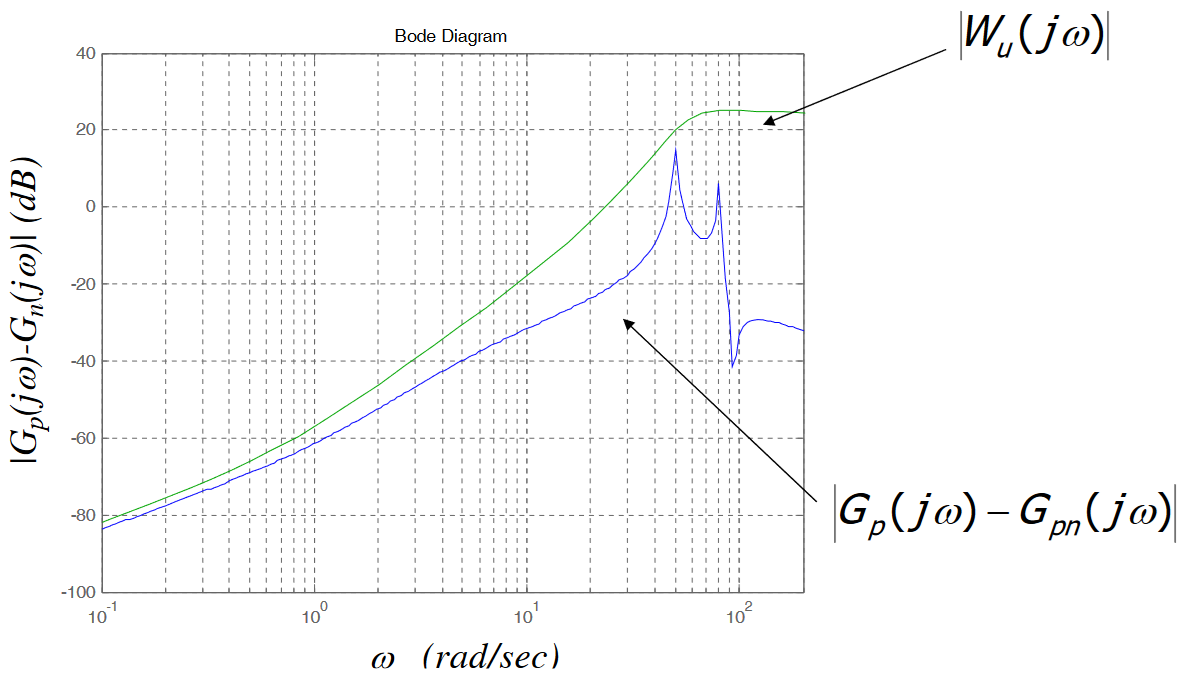
\includegraphics[width=0.6\textwidth]{images/additive_uncertainty.png}
		\caption{Weighting Function $W_u$ considering $M_a$}
		\label{fig:image6}
	\end{figure}
	
	\raggedright
	\subsubsection{Multiplicative Uncertainty}
	The multiplicative uncertainty model set is defined as:
	\begin{equation}
		M_m = \left\{ G_p(s): G_p(s)=G_{pn}(s) \left[1+W_u(s)\Delta(s)\right], \left\lVert\Delta(s)\right\rVert_\infty \leq1 \right\}
	\end{equation}
	where, by construction, the following condition must be satisfied by the weighting function $W_u(s)$:
	\begin{equation}
		\left\lVert \left( \dfrac{G_p(s)}{G_{pn}(s)}-1 \right) \dfrac{1}{W_u(s)}\right\rVert_\infty = \left\lVert \Delta(s) \right\rVert_\infty \leq 1
	\end{equation}
	which is equivalent to:
	\begin{equation}
		\left| \dfrac{G_p(j\omega)}{G_{pn}(j\omega)}-1 \right| \leq \left| W_u(j\omega) \right| \quad \forall \omega
	\end{equation}
	
	Below is an example of the frequency response of $W_u(j\omega)$ for a multiplicative uncertainty model set:
	
	\begin{figure}[H] % Use [H] to fix the position
		\centering
		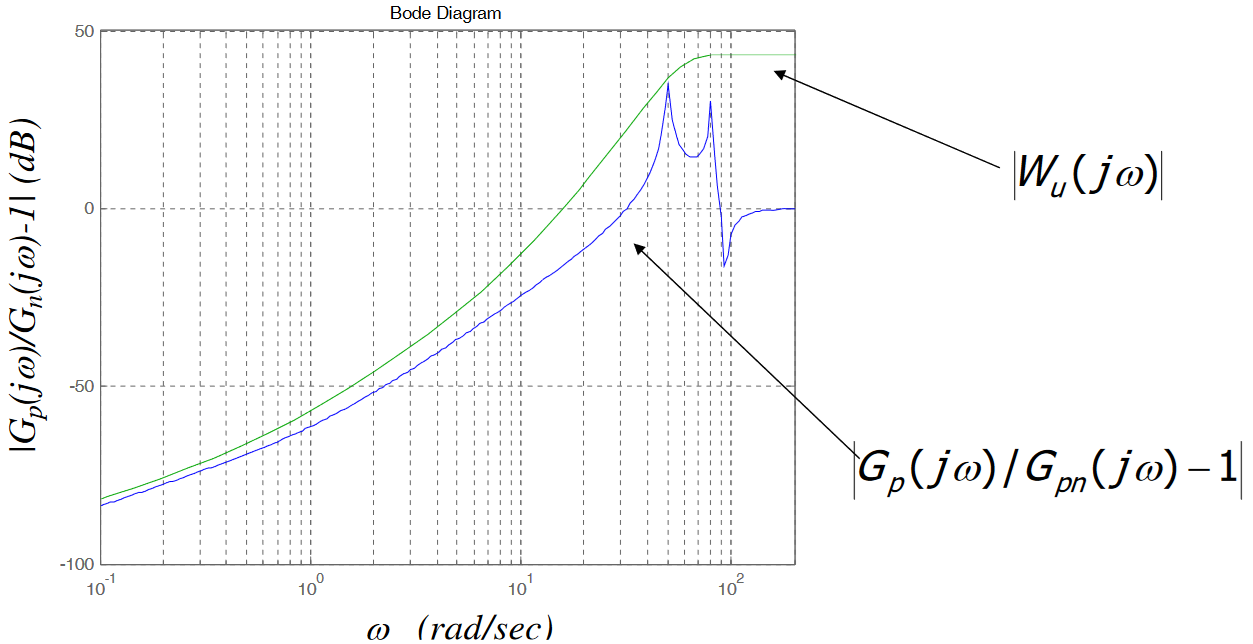
\includegraphics[width=0.68\textwidth]{images/multiplicative_uncertainty.png}
		\caption{Weighting Function $W_u$ considering $M_m$}
		\label{fig:image7}
	\end{figure}
	
	\raggedright
	Now we consider the problem of properly selecting the \textbf{nominal model} $\bm{G_{pn}}$ in order to \textbf{minimize} the size $W_u$ of the unstructured uncertainty of the given model:
	Let's consider, without loss of generality, the following nominal model:
	\begin{equation}
		G_{pn}(s) = \dfrac{K_n}{s-p}
	\end{equation}
	where $K_n$ is a constant value to be computed.
	The weighting function $W_u(s)$ must satisfy the following condition:
	\begin{equation}
		\left\lVert \Delta(s) \right\rVert_\infty = \sup_\omega \left| \left( \dfrac{G_p(j\omega)}{G_{pn}(j\omega)}-1 \right) \dfrac{1}{W_u(j\omega)} \right| \leq 1
	\end{equation}
	which is equivalent to:
	\begin{equation}
		\left| W_u(j\omega) \right| \geq \left| \dfrac{G_p(j\omega)}{G_{pn}(j\omega)}-1 \right| = \left| \dfrac{K}{K_n}-1 \right| \quad \forall\omega,\;\forall K 
	\end{equation}
	$K_n$ can be selected in order to minimize the size of the uncertainty in the following way:
	\begin{equation}
		\left| W_u(j\omega) \right| \geq \min_{K_n}\max_K \left| \dfrac{K}{K_n}-1 \right| \quad \forall\omega
	\end{equation}
	It can be easily shown that:
	\begin{equation}
		\min_{K_n}\max_K \left| \dfrac{K}{K_n}-1 \right| = \min_{K_n}\max \left\{\ \left| \dfrac{\overline{K}-K_n}{K_n} \right|, \left| \dfrac{\underline{K}-K_n}{K_n} \right| \right\}
	\end{equation}
	The solution is found at the intersection of the two functions to maximise (between curly braces in 7.1.11), and it is the following:
	\begin{equation}
		K_n = \dfrac{\overline{K}+\underline{K}}{2}
	\end{equation}
	
	\subsubsection{Inverse Additive Uncertainty}
	The inverse additive uncertainty model set is defined as:
	\begin{equation}
		M_{ia} = \left\{ G_p(s): G_p(s)= \dfrac{G_{pn}(s)}{1+W_u(s)\Delta(s)G_{pn}(s)}, \left\lVert\Delta(s)\right\rVert_\infty \leq1 \right\}
	\end{equation}
	\subsubsection{Inverse Multiplicative Uncertainty}
	The inverse multiplicative uncertainty model set is defined as:
	\begin{equation}
		M_{im} = \left\{ G_p(s): G_p(s)= \dfrac{G_{pn}(s)}{1+W_u(s)\Delta(s)}, \left\lVert\Delta(s)\right\rVert_\infty \leq1 \right\}
	\end{equation}
	
	\subsection{Conclusion and Remarks}
	An important remark is that \textbf{unstructured uncertainty model sets can only provide a conservative description of parametric uncertainties} since, as shown in the above example, a complex function $\Delta(s)$ is used to account for the source of uncertainty, which is a real number.
	The unstructured uncertainty model set describes, at each frequency $\omega$, the uncertainty as a disk of radius $\left| W_u(j\omega)L_n(j\omega) \right|$.
	
	\section{Unstructured Uncertainty Modelling and Robustness}
	The aim is to study the stability of a feedback control system under the assumption that $G_p$ is an uncertain system described by a given uncertainty model set. The following discussion will consider a multiplicative uncertainty model set $M_m$.
	
	\subsection{Robust Stability}
	The feedback control system displayed in Figure 1 is \textbf{robustly stable} if and only if it is internally stable for each $G_p$ which belongs to $M_m$.
	As a result, the following condition on the weighting function $W_u$ must be satisfied:
	
	\begin{equation}
		\left\lVert W_uT_n \right\rVert_\infty < 1
	\end{equation} 
	
	where $T_n$ is the \textbf{nominal complementary sensitivity function}.
	Robust stability conditions for every described uncertainty model set are shown in the table below:
	\begin{center}
		\vspace{2pt}
		\begin{tabular}{|c|c|}
			\hline
			\textbf{Uncertainty Model Set} & \textbf{Robust Stability Condition} \\ \hline
			$M_m$ & $\left\lVert W_uT_n \right\rVert_\infty < 1$ \\ \hline
			$M_a$ & $\left\lVert W_uG_cS_n \right\rVert_\infty < 1$ \\ \hline
			$M_{ia}$ & $\left\lVert W_uG_{pn}S_n \right\rVert_\infty < 1$ \\ \hline
			$M_{im}$ & $\left\lVert W_uS_n \right\rVert_\infty < 1$ \\ \hline
		\end{tabular}
	\end{center}
	In other words, we have to guarantee that the uncertainty does not change the number of encirclements of the point $-1$ in the Nyquist plot of the loop function:
	
	\begin{figure}[H] % Use [H] to fix the position
		\centering
		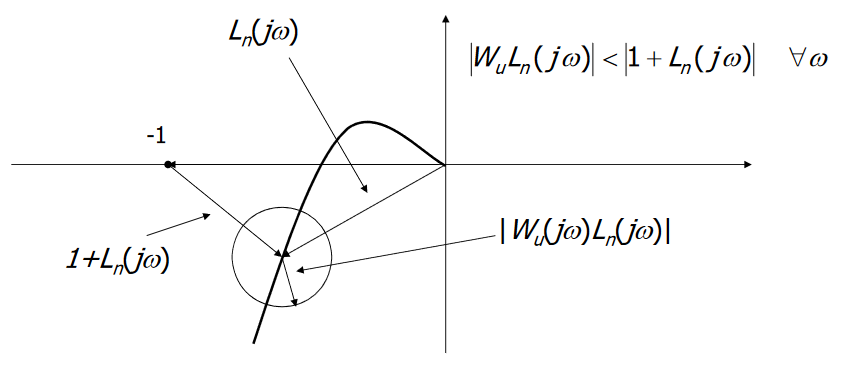
\includegraphics[width=0.6\textwidth]{images/robust_stability_proof.png}
		\caption{Nyquist Plot for Robust Stability Visualization}
		\label{fig:image8}
	\end{figure}
	
	\subsection{Nominal Performance}
	The nominal performance conditions, derived previously in subsection 6.1, are requirements affecting the sensitivity and complementary sensitivity functions as follows:
	
	\begin{equation}
		\left\lVert W_SS_n \right\rVert_\infty < 1 \iff \left| 1+L_n(j\omega) \right| > \left| W_S(j\omega) \right| \quad \forall\omega 
	\end{equation}
	\begin{equation}
		\left\lVert W_TT_n \right\rVert_\infty < 1 
	\end{equation}
	If we use the Nyquist Plot as before for visualization, the concept is very similar, but the "uncertainty disk" this time is centered around $-1$.
	
	\begin{figure}[H] % Use [H] to fix the position
		\centering
		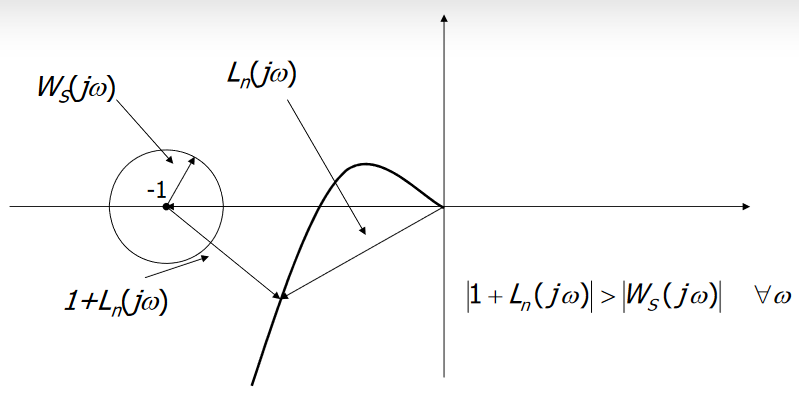
\includegraphics[width=0.6\textwidth]{images/nominal_performance_proof.png}
		\caption{Nyquist Plot for Nominal Performance Visualization}
		\label{fig:image9}
	\end{figure}
	
	\subsection{Robust Performance}
	The feedback system guarantees \textbf{robust performance} if and only if performance requirements are satisfied for each $G_p$ which belongs to the given uncertainty set.
	Considering the case in which performance requirements affect only the sensitivity function and uncertainty is described by means of a multiplicative uncertainty model set, the following condition must be satisfied (restricted to the case of $W_T = 0$):
	
	\begin{equation}
		\left\lVert \left| W_SS_n \right| + \left| W_uT_n \right | \right\rVert_\infty < 1
	\end{equation}
	The Nyquist Plot below allows for an easy visualization of the concept of Robust Performance, which is satisfied if and only if the two "uncertainty disks" do not overlap.
	
	\begin{figure}[H] % Use [H] to fix the position
		\centering
		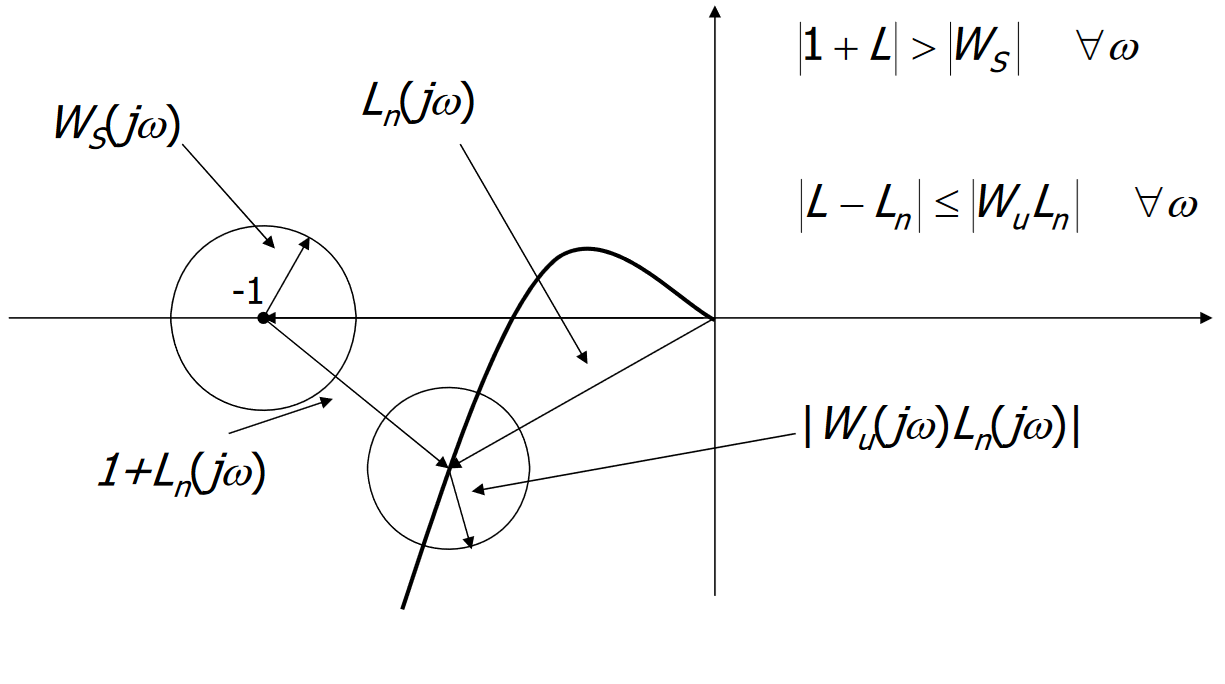
\includegraphics[width=0.6\textwidth]{images/RS_NP_proof.png}
		\caption{Nyquist Plot for Robust Performance Visualization}
		\label{fig:image10}
	\end{figure}
	
	\section{$\bm{H_\infty}$ Design for Robust Control}
	\subsection{Problem Definition}
	Given definition 6.1.2 for SISO LTI systems, the $H_\infty$ norm minimization approach, called $H_\infty$ control, refers to a general formulation of the control problem which is based on the following block diagram representation of a general feedback system:
	
	\begin{figure}[H]
		\centering
		\begin{minipage}{0.5\textwidth}
			\begin{enumerate}
				\item[$\bullet$] $\bm{M}$ is the \textbf{generalized plant}
				\item[$\bullet$] $\bm{G_c}$ is the controller
				\item[$\bullet$] $\bm{u}$ are the control inputs
				\item[$\bullet$] $\bm{v}$ are the controller inputs
				\item[$\bullet$] $\bm{w}$ are the external inputs
				\item[$\bullet$] $\bm{z}$ are the external outputs
			\end{enumerate}
		\end{minipage}%
		\begin{minipage}{0.3\textwidth}
			\centering
			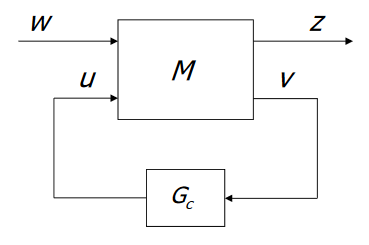
\includegraphics[width=\linewidth]{images/H_inf_feedback_CS.png}
			\caption{$H_\infty$ Feedback Control System Block Diagram.}
			\label{fig:image11}
		\end{minipage}
	\end{figure}
	The external inputs and output signals of the generalized plant are not necessarily physical variables of the control system and must be carefully selected in order to take into account the stability and performance requirements of the considered control problem.
	
	\subsection{Controller Design}
	In the $H_\infty$ design, the controller is obtained by solving the following optimization problem:
	\begin{equation}
		G_c(s) = \arg\min_{G_c \in G_c^{stab}} \left\lVert T_{wz}(s) \right\rVert_\infty 
	\end{equation}
	where $G_c^{stab}$ is the class of all the controllers which provide internal stability of the nominal feedback system, and $T_{wz}$ is the closed loop transfer function between the input $w$ and the output $z$.\\
	Therefore, the design of the controller is performed in three steps:
	
	\begin{enumerate}
		\item[$\bullet$] select the transfer function $T_{wz}$
		\item[$\bullet$] build the generalized plant $M$ corresponding to the selected $T_{wz}$.
		\item[$\bullet$] compute $G_c(s)$ by solving 9.2.1
	\end{enumerate}
	
	\subsubsection{Generalized Plant for Robust Stability}
	Let's consider the problem of designing a controller $G_c$ to robustly stabilize an uncertain system described by means of the unstructured multiplicative model set.\\
	The condition for robust stability is 8.1.1, and a controller that satisfies this condition can be found by choosing the following transfer function $T_{wz}$:
	
	\begin{equation}
		T_{wz}(s) = W_2T_n
	\end{equation}
	where $W_2(s) = W_u(s)$.
	
	\subsubsection{Generalized Plant for Nominal Performance}
	Let's consider the problem of designing a controller $G_c$ to satisfy the nominal performance conditions.\\
	The conditions for nominal performance are 8.2.1 and 8.2.2, and a controller that satisfies them can be found by choosing the following transfer function $T_{wz}$ as a \textbf{stack} of two transfer functions:
	
	\begin{equation}
		T_{wz}(s) = 
		\begin{bmatrix}
			W_1 S_n \\
			W_2 T_n
		\end{bmatrix}
	\end{equation}
	where $W_1(s) = W_S(s)$ and $W_2(s) = W_T(s)$.
	
	\subsubsection{Generalized Plant for Robust Stability and Nominal Performance}
	Finally, let's consider the problem of designing a controller $G_c$ that satisfies both conditions.\\
	Since the complementary sensitivity function must satisfy the following two frequency domain constraints:
	\begin{equation}
		\left| T_n(j\omega) \right| \leq \left| W_T^{-1}(j\omega) \right| \quad , \quad \left| T_n(j\omega) \right| \leq \left| W_u^{-1}(j\omega) \right| \quad \forall\omega
	\end{equation}
	$T_{wz}$ can be chosen as in 9.2.3, where in this case $W_1(s) = W_S(s)$ and $W_2(s)$ is such that for each $\omega$:
	\begin{equation}
		\left| W_2(j\omega) \right| = \max \left( \left| W_u(j\omega) \right| , \left| W_T(j\omega) \right| \right)
	\end{equation}
	
	For better visualization assume, without loss of generality, that $G_a=G_s=G_f=1$.\\
	The generalized plant $M$ corresponding to the selected transfer function $T_{wz}$ is the following:
	
	\begin{figure}[H] % Use [H] to fix the position
		\centering
		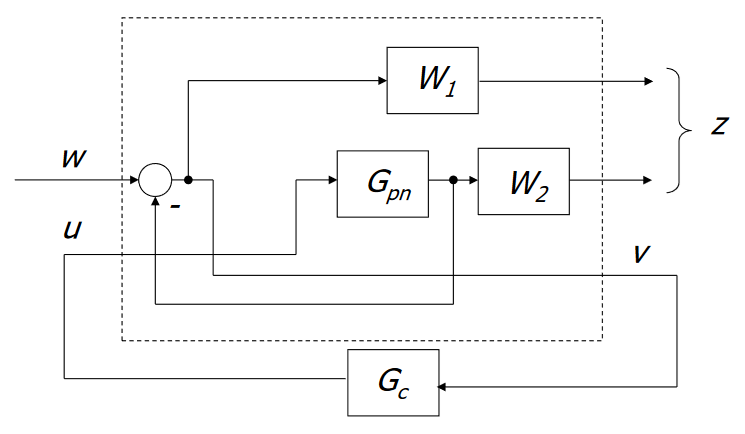
\includegraphics[width=0.6\textwidth]{images/generalized_plant.png}
		\caption{Generalized Plant Block Diagram.}
		\label{fig:image12}
	\end{figure}
	
	Control problems involving constraints on the $H_\infty$ norm on more than one closed loop transfer functions are called \textbf{mixed sensitivity problems}.\\
	The controller design problem obtained by applying the "stacking procedure" to a mixed sensitivity problem is referred to as a \textbf{stacked mixed sensitivity problem}.
	
	\subsection{LMI Optimization Approach}
	As previously stated, the $H_\infty$ controller is designed by solving equation 9.2.1.\\
	\vspace{2pt}
	Among the approaches proposed in the literature which solve such an optimization problem, this document will present one based on the solution of a suitable constrained optimization problem, where the constraints are in the form of linear matrix inequalities (LMI).\\
	\vspace{2pt}
	The LMI approach is based on a state-space description of the generalized plant M:
	
	\begin{figure}[H]
		\begin{minipage}{0.3\textwidth}
			\centering
			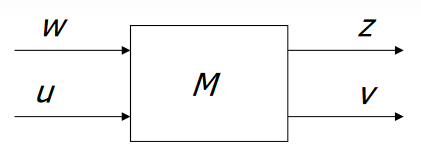
\includegraphics[width=\linewidth]{images/generalized_plant_small.png}
			\label{fig:image13}
		\end{minipage}
		\centering
		\begin{minipage}{0.5\textwidth}
			\vspace{-20pt}
			\begin{equation}
				\left\{
				\begin{aligned}
					\dot{x_M} &= Ax_M + B_1w + B_2u \\
					z &= C_1x_M + D_{11}w + D_{12}u \\
					v &= C_2x_M + D_{21}w + D_{22}u
				\end{aligned}
				\right.
			\end{equation}
		\end{minipage}
	\end{figure}
	where $\bm{X_M}$ \textbf{is the state of the generalized plant.} \\
	\vspace{2pt}
	The LMI optimization problem can be solved under the following assumptions:
	\begin{enumerate}
		\item[$\bullet$] The matrix triplet $(A,B_2,C_2)$ is stabilizable and detectable.
		\item[$\bullet$] $D_{22} = 0$ 
	\end{enumerate}
	
	\subsubsection{Internal stability of the generalized plant $\bm{M}$}
	Considering the mixed sensitivity problem, the generalized plant M can be internally stabilized by an LTI controller $G_c$ having input v and output u \textbf{if and only if} $W_1$ and $W_2$ are stable transfer functions.
	
	
	
	
	

\end{document}